% !Mode:: "TeX:UTF-8"
\documentclass{xcumcmart}
\usepackage{setspace}
\usepackage{enumerate}
% \title{text}这里是显示在第三页的文章标题
\title{基于线性模型的钢水“脱氧合金化”方案优化}
% \displaytitle{text}这里是显示在承诺书上的文章标题,注意,不能换行,如果题目特别长,要进行适当的缩写
\displaytitle{高教社杯全国大学生数学建模竞赛论文 \LaTeX{} 模板示例}
% \school{text}命令用于在承诺书上显示学校名称。按要求,此处应填写全称
\school{China\TeX{}大学}
% 以下命令分别显示队员及指导教师姓名
\authorone{Ch'en Meng}
\authortwo{Liam Huang}
\authorthree{ShadowInShadow}
\advisor{China\TeX{}}

\usepackage{metalogo,hyperref} % 这里加载的宏包仅仅是为了本示例文档,实际使用时可以根据需要删除。
\linespread{1.2} 
\begin{document}
\renewcommand\arraystretch{2}



\maketitle
\begin{cnabstract}%此处没有采用sbstract命名,是为了将来如果要加入英文摘要时扩展的方便
\setlength{\parskip}{1.4em}

\par \textit{占位文字,待替换题目需要我们通过对合金钢的生产历史数据进行分析,应该利用统计学知识以及数据处理的方法,对数据进行适当的预处理,再根据题目的具体要求,利用合理的指标和算法进行建模,并进行模型检验。}
\par \textbf{关键词:脱氧合金化 回归拟合 线性优化}
\end{cnabstract}
\setlength{\parskip}{1.4em}

%\tableofcontents\newpage%增加目录,要不要都可以。不想要的话,就在本行前加“%”(英文的百分号)
一篇典型的数模竞赛论文,通常包括以下部分,当然,这些并不全是必须的。
\section{问题重述}
\par 目前,各大钢铁企业为提高竞争力所要解决的重要问题是:如何在保证钢水质量的同时最大限度降低合金钢的生产成本。这要求我们通过历史数据对脱氧合金化环节建立数学模型,在线预测并优化投入合金的种类及数量,最终实现成本-收益最大化目标。我们需要通过题目所给数据解决如下问题:
\begin{enumerate}[(i)]%(\arabic{section}.1)
\item 计算C、Mn两种元素的历史收得率,并分析影响其收得率的主要因素。
\item 基于问题1,对C、Mn元素收得率进行预测,并对模型进行改进。
\item 基于问题2实现钢水脱氧合金化的成本优化计算,并给出合金配料方案。
\item 根据研究结果给炼钢厂提出建议。
\end{enumerate}

\section{问题分析}
\par 题目需要我们通过对合金钢的生产历史数据进行分析,应该利用统计学知识以及数据处理的方法,对数据进行适当的预处理,再根据题目的具体要求,利用合理的指标和算法进行建模,并进行模型检验。
\par 问题一要求我们根据历史数据测算出C、Mn两种元素的历史收得率。计算之前应对数据的缺失情况进行分析,并合理地进行缺失值按行或按列丢弃、均值替代等操作,保证计算的可靠性。针对收得率影响因素的研究,首先使用相关系数进行定性的初步判定,其次增加线性回归进行定量分析。
\par 问题二要求我们对收得率进行预测,并改进模型及算法提高预测的准确性。第一题线性模型可以实现对元素收得率的预测,在此基础上模型改进有以下两点:第一,进一步确定元素收得率在实际工业应用中的可能影响因素,考虑数据缺失情况以及预测模型的需要,处理缺失值较多的变量时,将转炉终点缺失值替换为均值,重新计算收得率;第二,使用多种回归算法,通过合理的回归评价指标确定最佳模型算法。
\par 问题三是目标函数最优化问题,利用第二问的预测模型稍加修改,可实现对连铸合金的元素含量预测,根据题目所给HRB400B型号合金钢的元素含量标准建立线性约束,由于仅需要优化配料的成本,将未知的转炉终点元素含量以及转炉终点温度、钢水质量等无关变量全部使用均值替代,最终建立价格目标函数求解满足条件的最优方案。
\par 问题四则为基于上述问题的分析结果提出本团队的生产建议。

\section{假设与符号}

\section{模型的建立与求解}
\subsection{问题一的解答}
\subsubsection{问题一的分析}
\par 由题目可得,合金收得率是指脱氧合金化时被钢水吸收的合金元素的重量与加入 该元素总重量之比。转炉终点指脱氧合金化之前钢水中某个元素的含量,连铸正样为脱氧合金化之后钢水中该元素的含量,因而被吸收的合金元素重量可用连铸正样与转炉终点的差值表示,再除以加入的该元素总重量即可求得历史收得率。通过分别分析各变量与C、Mn之间的相关系数初步判断合金收得率的影响因素,其次通过构建线性回归与归一化进行定量分析,最终得出收得率的影响因素。
\subsubsection{数据描述与预处理}
\par 附件一中的数据主要包括转炉终点各元素含量、连铸正样各元素含量以及加入合金配料质量、钢水总质量等数据项。
\par 部分变量的缺失值较多,例如:C、Mn元素连铸正样只有906组历史采样数据。因此将未采样的连铸正样数据行丢弃。
\par 如图\ref{fig:prev},通过直方图和折线图可以看到数据中存在离群值,且数据大致呈正态分布,为了提高分析的可靠性,需要将离群值去掉,仅保留$[\mu-3\sigma,\mu-3\sigma]$范围类的数据,根据正态分布3$\sigma$原则,该范围理论上包括99.73\%的原始数据。
\begin{figure}[htbp]
	\centering
	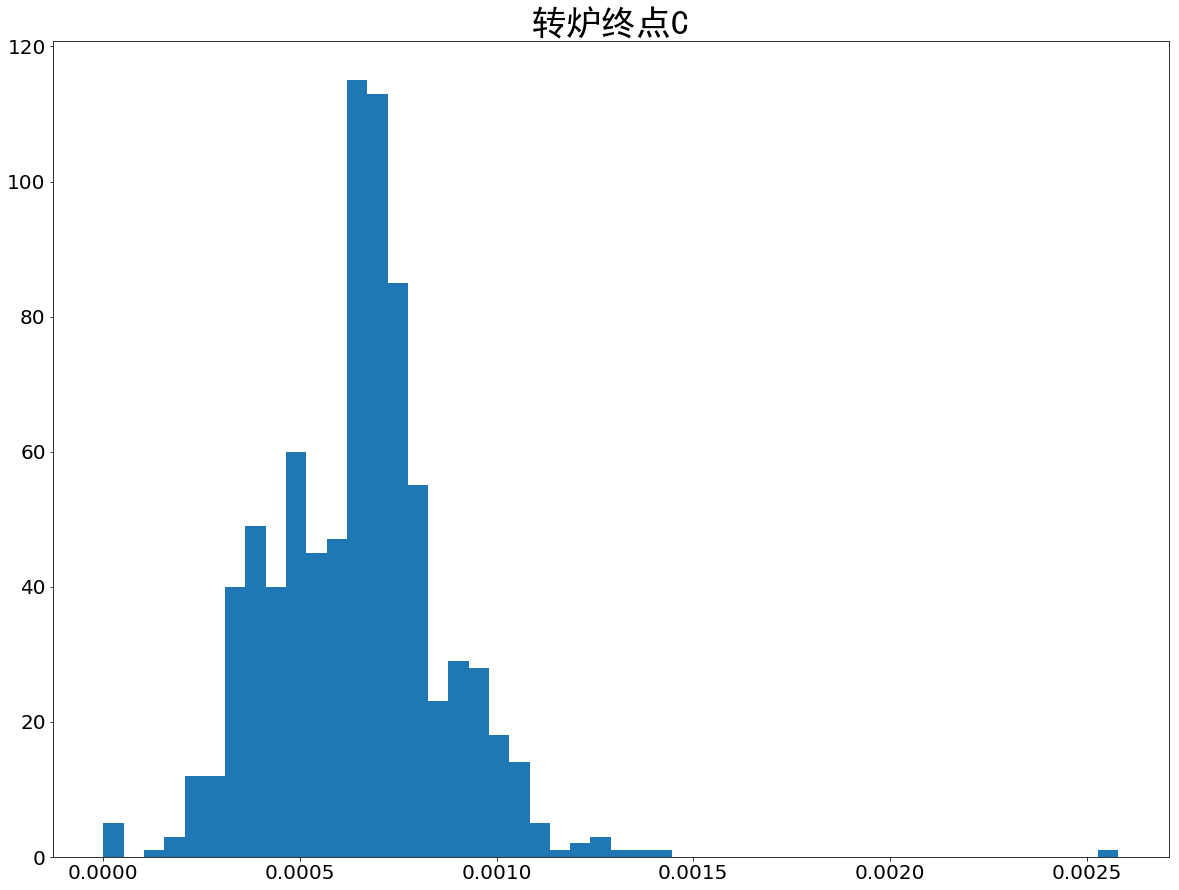
\includegraphics[width=0.45\textwidth]{fig/hist.png}
	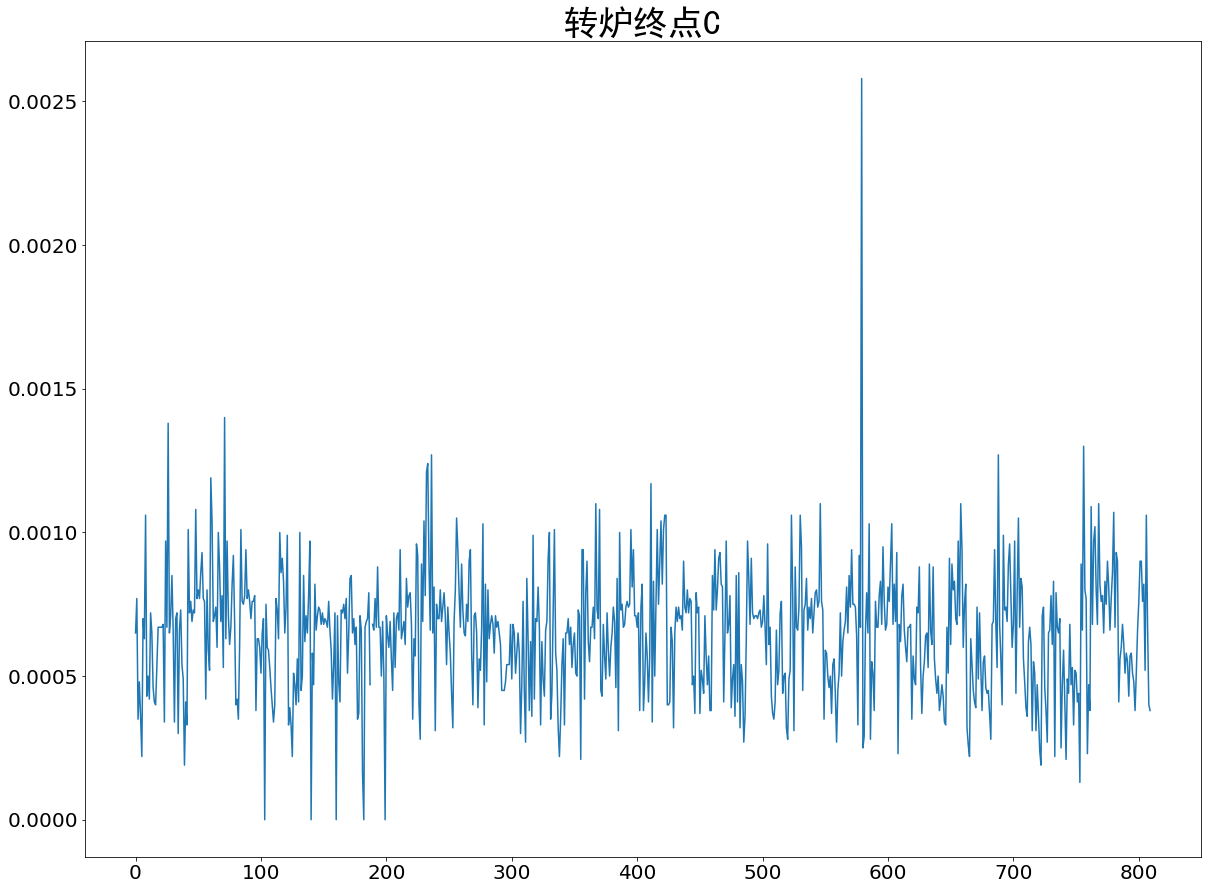
\includegraphics[width=0.45\textwidth]{fig/index.png}
	\caption{转炉终点C的数据分布\label{fig:prev}}
\end{figure}
\subsubsection{历史收得率的计算}
由题目可得,合金历史收得率的计算公式为:
\begin{equation} \label{eq:eps1}
    H_i=\frac{M(Out_i-Beg_i)}{T_i}\times 100\%
\end{equation}
  其中,$T_i$为添加配料中元素i的总质量,计算方式为$T_i=C_{i}^{T}X$,$X$为加入配料的质量构成的向量,$C_i$为每种配料对应元素i的含量。
$Beg_i$、$Out_i$分别为脱氧合金化前后钢水中元素i的含量。计算得到的历史收得率见附录。

\subsubsection{收得率影响因素分析}
相关系数(Correlation coefficient)是反应变量之间关系密切程度的统计指标,相关系数的取值区间在1到-1之间。1表示两个变量完全线性相关,-1表示两个变量完全负相关,0表示两个变量不相关。数据越趋近于0表示相关关系越弱。公式\ref{eq:eps2}是相关系数的计算公式:
\begin{equation} \label{eq:eps2}
    r_{xy}=S_{xy}/(S_xS_y )
\end{equation}

其中$r_{xy}$ 表示样本相关系数,$S_{xy}$ 表示样本协方差,$S_x$ 表示$x$的样本标准差,$S_y$  表示$y$的样本标准差。下面分别是$S_{xy}$协方差和$S_x$和$S_y$标准差的计算公式。由于是样本协方差和样本标准差,因此分母使用的是$n-1$。
\[S_{xy}=\frac{\sum{i=1}^n(X_i-\overline{X})(Y_i-\overline{Y})}{n-1}\]
\[S_x=\sqrt{\frac{(X_i-\overline{X})^2}{n-1}}\]
\[S_y=\sqrt{\frac{(Y_i-\overline{Y})^2}{n-1}}\]
本团队分别计算了脱氧合金化过程中与该元素相关的变量与该元素收得率之间的相关系数,并保留了相关系数绝对值大于0.1的影响因素,具体数据见下图:

\section{模型的检验}
\section{进一步讨论}
\section{模型的优缺点}

\begin{thebibliography}{1}
\bibitem{1} 全国大学生数学建模竞赛组委会, 2004 高教社杯全国大学生数学建模竞赛论文格式规范, 2004
\bibitem{2} 全国大学生数学建模竞赛组委会, 2013 高教社杯全国大学生数学建模竞赛论文格式规范, 2013
\end{thebibliography}

\end{document}
